\usetikzlibrary{topaths,calc}

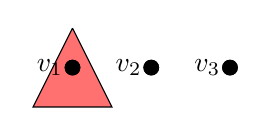
\begin{tikzpicture}
    \node (v1) at (-1,0) {};
    \node (v2) at (0,0) {};
    \node (v3) at (1,0) {};

    \begin{scope}[fill opacity=0.8]
    \filldraw[fill=red!70]
        ($(v1)+(0.0,0.5)$)
        to ($(v1)+(-0.5,-0.5)$)
        to ($(v1)+(0.5,-0.5)$)
        to ($(v1)+(0.0,0.5)$);
    \end{scope}


    \foreach \v in {1,2,3} {
        \fill (v\v) circle (0.1);
    }

    \fill (v1) circle (0.1) node [left] {$v_1$};
    \fill (v2) circle (0.1) node [left] {$v_2$};
    \fill (v3) circle (0.1) node [left] {$v_3$};

\end{tikzpicture}
